\documentclass[12pt,Chicago,final]{uuthesis2e}
\pdfpagewidth 8.5truein
\pdfpageheight 11.0truein
%\documentclass[12pt,Chicago,draft]{uuthesis2e}
\usepackage[%
labelsep=period
]{caption}
\usepackage{uuthesis-2013}
\usepackage{ifpdf}
\raggedbottom

%\usepackage[nooneline]{subfigure}
\usepackage{hyphenat}
\usepackage{afterpage}

\usepackage[sectionbib,numbers]{natbib} % numeric citations

\usepackage{color}
\usepackage{mathptmx}

\usepackage{times}

\usepackage{amssymb}
\usepackage{eepic}
\usepackage{marvosym}
\usepackage{verbatim}
\usepackage{alltt}

\usepackage{amsmath}
\usepackage{amsfonts}
\usepackage{mathptmx}
\usepackage{url}
\usepackage{pxfonts}

\usepackage{multirow}
\usepackage{moreverb}
\usepackage{subfig}
\usepackage{listings}
\usepackage{lscape}
\usepackage[all]{nowidow}
\usepackage{booktabs}
\usepackage{import}
\usepackage{hhline}% http://ctan.org/pkg/hhline
\ifpdf
	\usepackage[pdftex]{graphicx}
	\pdfcompresslevel=9
	\DeclareGraphicsExtensions{{.png},{.pdf},{.jpg},{jpeg}}
	\graphicspath{ {png/} {jpg/} {pdf/} {Figures/} }
	\usepackage[final]{pdfpages}
\else
	\usepackage[dvips]{graphicx}
	\DeclareGraphicsExtensions{.eps}
	\graphicspath{ {fig/} {eps/} }
\fi

\usepackage{mwe,tikz}\usepackage[percent]{overpic}
\usetikzlibrary{shadows}
\usepackage{rotating} % Provides {sideways}{sidewaysfigure}{sidewaystable} environments

%%
\usepackage{color}
\definecolor{rltbrightred}{rgb}{1,0,0}
\definecolor{rltred}{rgb}{0.75,0,0}
\definecolor{rltdarkred}{rgb}{0.5,0,0}
%
\definecolor{rltbrightgreen}{rgb}{0,0.75,0}
\definecolor{rltgreen}{rgb}{0,0.5,0}
\definecolor{rltdarkgreen}{rgb}{0,0,0.25}
%
\definecolor{rltbrightblue}{rgb}{0,0,1}
\definecolor{rltblue}{rgb}{0,0,0.75}
\definecolor{rltdarkblue}{rgb}{0,0,0.5}

\newenvironment{figure*}
{\begin{figure}}
{\end{figure}}

\begin{comment}
\usepackage
[
bookmarksopen=true,
%linktocpage,
colorlinks=true,
urlcolor=rltdarkblue,                % \href{...}{...}
filecolor=rltdarkblue,              % \href*{...}
linkcolor=rltdarkblue,                % \ref{...} and \pageref{...}
citecolor=rltdarkblue,        % \cite{...}
anchorcolor=rltdarkblue,       % ???
menucolor=rltdarkblue,           % ??? 
]
{hyperref} 
\end{comment}

\usepackage[chapter]{algorithm}
\usepackage{algpseudocode}
\usepackage{amssymb}

\newcommand{\torsoname}{torso\_29yo}
\newcommand{\torsocnt}{2.74M}
\newcommand{\VEC}[2]{\mathbf{#1}_{#2}}
\newcommand{\etal}{\textit{et al.}}
\DeclareMathOperator\ShiftLeft{\texttt{<<}}% shift left
\DeclareMathOperator\ShiftRight{\texttt{>>}}% shift left




\usepackage{siunitx}
% group comma separator for large numbers
\sisetup{group-separator = {,}}

\usepackage{pgfplots}
\usepackage{pgfplotstable}

\pgfplotstableread[col sep=comma]{movingsurfaces_tex/data.txt}\mytable
\def\getcell#1#2#3{
	\pgfplotstablegetelem{#1}{#2}\of{#3}\pgfplotsretval%
}

\pgfplotstableread[col sep=comma]{movingsurfaces_tex/data-neighbor-idx.csv}\neighidx
\def\getcell#1#2#3{
	\pgfplotstablegetelem{#1}{#2}\of{#3}\pgfplotsretval%
}

\newcommand{\plotfile}[1]{
	\pgfplotstableread{#1}{\table}
	\pgfplotstablegetcolsof{#1}
	\pgfmathtruncatemacro\numberofcols{\pgfplotsretval-1}
	\pgfplotsinvokeforeach{1,...,\numberofcols}{
		\pgfplotstablegetcolumnnamebyindex{##1}\of{\table}\to{\colname}
		\addplot table [y index=##1] {#1}; 
		\addlegendentryexpanded{\colname}
	}
}

%\usepackage{cite}
\citeindextrue
\makeindex
%\includeonly{chapter1}
\title{GPU-Enabled Surface Visualization}

\author{Mark Kim}

%\thesistype{proposal}
\thesistype{dissertation}

\degree{Doctor of Philosophy}

\graduatedean{David S. Chapman}
\department{School of Computing}
\departmentchair{Ross Whitaker}
\committeechair{Charles D. Hansen}
\chairtitle{Professor}
\firstreader{Christopher Johnson}
\secondreader{Mike Kirby}
\thirdreader{Ross Whitaker}
\fourthreader{Guoning Chen}

\submitdate{May 2016}
\copyrightyear{2016}

% chapter is one level, section and subsection are the next two levels
\fourlevels

%% Dedication page
\dedication{}

%\inputpicturetrue % By Jeff McGough. See uuguide and private thesis.sty
%\inputpicturefalse % To NOT produce pictures, uncomment this line

%\newcommand{\BM }[1] {\mbox{\boldmath $#1$}}  

%%%%%%%%%%%%%%%%%%%%%%%%%%%%%%%%%%%%%%%%%%%%%%%%%%%%%%%%%%%%%%%%%%%%%%%%%%%%%%%%%%%%%%
% For shortening citations in the bibliography that are greater than six to et al.
% Since I am not using IEEE as my class, I need to declare this function.
% http://tex.stackexchange.com/questions/164017/limiting-the-number-of-authors-in-the-references-with-ieeetran
% http://tex.stackexchange.com/questions/16506/bibliography-author-initial-spacing
%%%%%%%%%%%%%%%%%%%%%%%%%%%%%%%%%%%%%%%%%%%%%%%%%%%%%%%%%%%%%%%%%%%%%%%%%%%%%%%%%%%%%%
\makeatletter
\def\bstctlcite{\@ifnextchar[{\@bstctlcite}{\@bstctlcite[@auxout]}}
\def\@bstctlcite[#1]#2{\@bsphack
	\@for\@citeb:=#2\do{%
		\edef\@citeb{\expandafter\@firstofone\@citeb}%
		\if@filesw\immediate\write\csname #1\endcsname{\string\citation{\@citeb}}\fi}%
	\@esphack}
\makeatother

\begin{document}
%%%%%%%%%%%%%%%%%%%%%%%%%%%%%%%%%%%%%%%%%%%%%%%%%%%%%%%%%%%%%%%%%%%%%%%%%%%%%%%%%%%%%%%
% NOTE: This function is declared above. It is used to control the 
% IEEEtrans bibliography bst.
% See the dissertation.bib for the @IEEEtranBSTCTL that forces the use 
% of et al. for author count greater than six.
% http://tex.stackexchange.com/questions/164017/limiting-the-number-of-authors-in-the-references-with-ieeetran
% http://tex.stackexchange.com/questions/16506/bibliography-author-initial-spacing
%%%%%%%%%%%%%%%%%%%%%%%%%%%%%%%%%%%%%%%%%%%%%%%%%%%%%%%%%%%%%%%%%%%%%%%%%%%%%%%%%%%%%%%
\bstctlcite{IEEEexample:BSTcontrol}
%change how figures are named
\renewcommand{\topfraction}{1.0}
\renewcommand{\bottomfraction}{1.0}
\renewcommand{\textfraction}{0.2}
\renewcommand{\floatpagefraction}{1.0}

\setcounter{bottomnumber}{1}
\setcounter{topnumber}{3}

%% Front matter
\frontmatterformat
\titlepage
\copyrightpage
\statementofapproval
%Thesis office doesn't need committee and reading pages since it should have the "real" copy.
%\committeeapproval
%\readingapproval

%% Abstract page
\preface{chapter_abstract}{Abstract}

\setcounter{page}{3}

%% Dedication page
%\dedicationpage

%% Table of contents, etc.
\tableofcontents
\listoffigures
\listoftables

%\optionalfront{Notation and Symbols}{\input{notation.tex}}

% Acknowledgments page.
\preface{chapter_acknowledgements}{Acknowledgements}
%\preface{intro}{Introduction}

\maintext % start normal page numbering, parts and chapters follow
\newcommand{\markmarker}[1]{{#1}}

\chapter{Introduction}\label{chapt:intro} 
%\section{Motivation}
Surface visualization is a fundamental technique in scientific visualization that facilitates understanding of surface data. It covers a wide range of data types and techniques, from mathematical algebraic surfaces to raster data and volume rendering to mesh extraction. Regardless of data type, though, there is usually a need for sophisticated but fast techniques. Further, surface visualization can be used as part of an iterative process to explore data sets. This iterative process requires a reasonable turnaround time for generating results because a lengthy turnaround time inhibits exploration of the data set.
As sophisticated surface visualization techniques are used to increase the quality of the output, in contexts such as medical imaging~\cite{PE.VMLS.VMLS2013.049-053} or surface flow visualization~\cite{SCI:Kim2015a}, these techniques come with an additional computational cost. That sophistication can also increase the amount of time it takes to iterate scientific discovery in a timely but accurate manner~\cite{Swe2012}. But this sophistication is key to accurate understanding of the data and cannot be discarded for performance. To address these issues, we developed new parallel techniques for surface visualization.

Surface visualization aids in the understanding of surface data, and in this dissertation we focus on two areas: conformal meshing with particles and unsteady surface flow visualization. Bioengineers need conformal, multimaterial meshes for accurate simulation~\cite{SCI:Swe2010a}.  In contrast to meshing, unsteady flow visualization, such as UFLIC, help engineers understand the flow on surfaces over time.  Although with very different purposes, both of these research areas have similar needs for exploring their data in a timely manner while maintaining the accuracy of the results. Additionally, surface visualization covers a broad spectrum of data types and techniques. Three-dimensional structured scalar data, such as those generated from magnetic resonance imaging (MRI) or computed tomography (CT), are frequently used in biomedical research for electrophysiological modeling. To conduct the modeling, a tetrahedral mesh is extracted from the structured data using a software package called BioMesh3D~\cite{SCI:BioMesh3D}. To perform accurate electrophysiological modeling, the mesh needs to be a conformal, high-quality multimaterial tetrahedral mesh~\cite{SCI:Swe2010a}. An example of a five-compartment mesh used in electrophysiology is in Fig.~\ref{fig:brainmeshing}. In contrast to a structured, three-dimensional scalar field, surface flow visualization often uses a triangular mesh with a velocity field sampled at the mesh vertices. With a velocity field represented in the mesh, various surface flow techniques are applied to visualize the field, such as line integral convolution (LIC), which has a physical analog:  placing oil onto aircraft to visualize flow separation (Fig.~\ref{fig:oilseparation}). Although dissimilar in structure and purpose, both multimaterial meshing and the surface flow visualization share a similar problem: sophisticated visualization techniques have a high computational cost for accurate visualization.

\begin{figure}[!b]
	\begin{center}
	\subfloat[]{%
	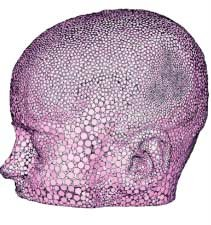
\includegraphics[height=1.5in]{images/brainmeshing1}
	\label{subfig:brainmeshing1}}
	\subfloat[]{%
	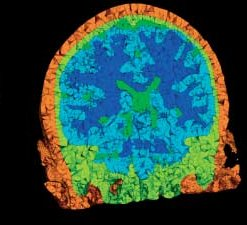
\includegraphics[height=1.5in]{images/brainmeshing2}
	\label{subfig:brainmeshing2}}
	\subfloat[]{%
	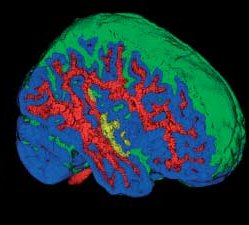
\includegraphics[height=1.5in]{images/brainmeshing3}
	\label{subfig:brainmeshing3}}

	\end{center}
	\caption{Five-compartment tetrahedral mesh using BioMesh3D. Fig.~\protect\subref{subfig:brainmeshing1} visualizes the particles on the surfaces. Figure~\protect\subref{subfig:brainmeshing2} and~\protect\subref{subfig:brainmeshing3} visualize the tetrahedral mesh. (MacLeod \textit{et al.}~\cite{SCI:Mac2009a})}
	\label{fig:brainmeshing}
\end{figure}

\begin{figure}[!t]
	\begin{center}
		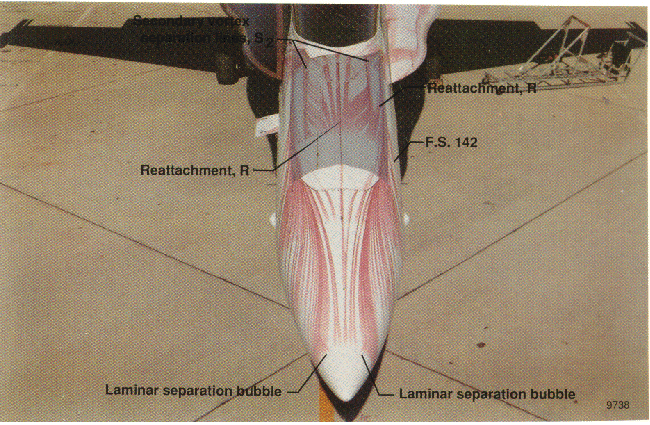
\includegraphics[width=5.0in]{images/f-18_inflight_oil_flow2}
		%Researchers at NASA's Langley Research Center in Hampton, Va., use all sorts of tools and techniques to learn more during the development of aircraft and spacecraft designs.
		%In this photo, engineers led by researcher Greg Gatlin have sprayed fluorescent oil on a 5.8 percent scale model of a futuristic hybrid wing body during tests in the14 by-22-Foot Subsonic Wind Tunnel.
		%The oil helps researchers "see" the flow patterns when air passes over and around the model. Those patterns are important in determining crucial aircraft characteristics such as lift and drag.
		%Image Credit: NASA Langley/Preston Martin 
	\end{center}
	\caption{In-flight oil flow ~\cite{inflightflowvis} (NASA~\cite{inflightflowvis}).}
	\label{fig:oilseparation}
\end{figure}

Surface visualization, and scientific visualization in general, is often used as part of an iterative data exploration process. This iterative data exploration process is a process of trial and error to explore the data. For example, in BioMesh3D there are user parameters to control some aspects of the mesh generation. If the turnaround time is lengthy, in practice this can lead to users resisting a technique or being unable to fully explore the data to generate an optimal solution. Therefore, it is preferable that surface visualization techniques be fast enough for users to iterate over their parameter space in a timely manner. At the same time, the high-quality results from the sophisticated techniques need to be maintained.

Users such as bioengineers or computational fluid dynamicists require increasingly sophisticated surface visualization for more accurate results, and this requirement increases computation time. The type of conformal multimaterial meshes used for biomedical electrophysiological modeling comes with a high computational cost, on the order of hours, or even days, to generate, that inhibits the ability of biomedical engineers to generate many models over time~\cite{Swe2012}. Similarly, state of the art in parameterized surface flow visualization, Flow Charts, requires a lengthy preprocess step to generate a parameterized surface upon which to perform unsteady flow line integral convolution~\cite{10.1109/TVCG.2008.58}. These lengthy times to generate results can interfere with the iterative nature of using surface visualization as an exploratory tool for data sets. But these techniques are crucial to their users for high-quality scientific discovery.

To address these issues, new parallel techniques were developed to be used in combination with general purpose computing on the graphics processing unit (GPGPU) to speed up surface visualization. At the same time, care is taken to retain the sophistication, complexity, and accuracy of the techniques that are required to continue to be useful for practitioners in their field.  This chapter continues with an overview of the contributions in this dissertation for surface visualization.

\section{Particle-Based Mesh Extraction on the GPU}
Isosurface extraction from three-dimensional scalar volumes is a fundamental technique in visualization. In some cases, the scalar data may be composed of different materials, and although the material is stored in a regular grid, the \markmarker{material interfaces} generally do not conform to the underlying grid. Meyer \textit{et al.}~\cite{SCI:Mey2007b,SCI:Mey2008a} introduced a particle-based approach to extract a conformal, curvature-dependent, well-formed multimaterial mesh from biological data. This approach used an energy-based system to extract a surface mesh with nearly equilateral triangles. Further, it generated meshes with smaller triangles in areas of high curvature, which gives more resolution in areas that need it. Well-formed triangular meshes are a good starting point to generate a tetrahedral mesh that is well suited for finite element simulation.

BioMesh3D~\cite{SCI:BioMesh3D} is a tool based on the research of Meyer \textit{et al.} and packaged into a pipeline for biological mesh extraction~\cite{SCI:Cal2009a}. However, due to the computational complexity of the particle advection process, users are required to find a balance between the heavy computation required and their needs in terms of the quality of the mesh, the quantity of tetrahedrons, and the time anticipated to extract the mesh. The excessive computational cost to generate a well-shaped multimaterial mesh has hindered the use of the curvature-dependent particle system by the bioengineering community for numerical simulations~\cite{SCI:Swe2010a}. For instance, an attempt was made to extract a mesh from a six-material dataset, but was finally stopped after two months because it had yet to finish~\cite{Swe2012}. Improving the performance could increase the use of the particle system for multimaterial mesh extraction and for various numerical simulation tasks.

We introduced a novel implementation of a particle system on the graphics processing unit (GPU) to reduce the run-time of the particle system. The adaption of a particle system to the GPU is inherently difficult due to the  single instruction multiple threads (SIMT) nature of the hardware. We studied the potential parallelization of the particle placement and proposed a simple strategy, called the red-black update, to segment the particles into groups that can be processed concurrently. Then, we explored the parallel feature provided by the recent advance of CUDA programming on the GPU, which allowed us to parallelize the computations when processing each particle in a group. Finally, we applied our GPU-based particle system to a number of medical datasets. The obtained meshes have comparable quality to those generated using a CPU-based particle placement, whereas the computation of our implementation is at least one order of magnitude faster than the CPU version for most cases, which is described in detail in Chapter~\ref{chapt:particle-system}.

\section{Enhanced Particle-Based Mesh Extraction}
The red-black update scheme achieved up to an order of magnitude speed-up for isosurface extraction using a single distance field on the GPU. Although it performed well on the GPU, unfortunately, it is not a natural mapping to the SIMT architecture. Further, extending the red-black scheme to multiple materials was problematic because of the SIMT nature of the GPU. The surface representation, a distance field, requires a reprojection step realized through an iterative root-finding algorithm to place particles back onto the surface. This reprojection step is inefficient on the GPU due to the amount of control flow, and forced the red-black update to run inefficiently on the GPU. Therefore, a new approach is needed to overcome these issues. We used the closest point embedding to define the surfaces in the volume for faster reprojection. We adapted the Barnes-Hut tree code, an octree-based acceleration structure, to speed up the particle energy calculation. Finally, new seeding and add/delete algorithms were developed to efficiently place new particles. 

\section{Surface Flow Visualization}
Vector field visualization is a fundamental technique in scientific visualization and is important in numerous scientific and engineering fields, such as computational fluid dynamics. One popular approach is line integral convolution (LIC)~\cite{Cabral:1993:IVF:166117.166151} because of its efficient utilization of the graphics processor as well as its ability to be used on surfaces embedded in three dimensions. 

Computing LIC on surfaces can be done in two ways: image-space methods and surface parameterization methods. Image-space methods generate LIC images on the visible parts of the surface~\cite{DBLP:conf/visualization/LarameeJH03,DBLP:conf/visualization/Wijk03}. In particular, the visible surface geometry and velocity field are projected onto the screen, and LIC is applied in the image space. By processing only the visible parts, the computation is highly interactive due to the GPU-generated LIC. Unfortunately, there are issues with image-space methods. Because only the visible geometry is processed, artifacts from altering the camera position can be noticed around silhouette edges or self-occluded areas of the mesh. 

Parameterizing the surface is another way to generate LIC on surfaces. Li \textit{et al.} achieved interactive frame rates rendering unsteady flow by partitioning the mesh into patches that are then packed into a texture atlas~\cite{10.1109/TVCG.2008.58}. Partitioning the mesh into patches is considered a preprocess step that is very time consuming.

To avoid the artifacts from image-space methods while at the same time addressing the lengthy preprocess step of Flow Charts, we presented a new method for unsteady flow line integral convolution (UFLIC) on a surface. Our parameterized space, the closest point embedding, came from the closest point method a simple but powerful technique for solving PDEs on embedded surfaces~\cite{DBLP:journals/jcphy/RuuthM08}. By using the closest point embedding, the parameterized surface was generated at near-interactive rates and the UFLIC was done at interactive rates, which allowed for flow visualization without the drawbacks of previous methods. To perform the flow visualization, a sparse closest point embedding was constructed by converting the triangular mesh into a coarse three-dimensional closest point grid. Once the closest point embedding was constructed, a refined grid and a neighborhood index are constructed to visualize the flow. Finally, an unsteady flow technique, UFLIC, was run over the refined grid to visualize the flow field.

\section{Surface Flow Visualization and the Closest \newline Point Sparse Octree}
Finally, as datasets continue to grow larger, new methods are needed to visualize them. To address this issue, we introduced the closest point sparse octree~\cite{SCI:Kim2016a}. By using a sparse octree instead of a structured grid, we could construct a closest point embedding up to $8,192^3$ in size on the GPU. Further, previously the closest point embedding was used to keep particles on the surface to perform UFLIC on the surface. However, by using the closest point method, particles no longer are kept on the surface to advect the noise. By extending the surface velocities and values into the surrounding grid and advecting the particles in the three-dimensional grid, the UFLIC is performed on the surface thanks to the \emph{equivalence of gradients}~\cite{DBLP:journals/jcphy/RuuthM08}.

%\section{Thesis Statement}

\section{Contributions}
\label{sec:contribution}
This dissertation explores speeding up surface visualization through the use of the GPU with the closest point embedding. The following contributions have been made:
\begin{itemize}
\item \textit{Particle System for Meshing on the GPU}. The curvature-dependent particle system~\cite{SCI:Mey2007b} is adapted to the GPU for isosurface mesh extraction~\cite{SCI:Kim2012}. A red-black Gauss-Seidel update method was developed to process bins of particles in parallel. This method achieved up to 44x speed-up over a CPU version.
\item \textit{Particle Mesh Extraction With the Closest Point Embedding and the GPU}. Unfortunately, the GPU particle system in~\cite{SCI:Kim2012} had some limitations. Although it achieved an order of magnitude speed-up over a CPU implementation, nevertheless it was difficult to implement and extend to multiple materials, and work load balancing was restricted. To remedy this, a tree code is used instead of binning to increase performance by not limiting the acceleration structure by the largest local feature size value. Further, a closest point embedding surface is used instead of multiple distance fields to immediately project the particle back onto the surface. By choosing the closest point embedding, multiple projections onto the surface are no longer needed~\cite{SCI:Kim2015b}.
\item \textit{Surface Flow Visualization Using the Closest Point Embedding}. The closest point embedding is a powerful tool to represent surfaces. Therefore, it is applied to surface flow visualization~\cite{SCI:Kim2015a}. Previous surface flow visualization attempts are either at least an order of magnitude too slow to parameterize the surface in near real-time or image-space based and unable to support techniques such as dye advection~\cite{Li:2006:GIA:2384796.2384800,DBLP:conf/visualization/LarameeJH03,DBLP:conf/visualization/Wijk03}. The closest point embedding is constructed in near real-time, and UFLIC~\cite{663898, Li:2006:GIA:2384796.2384800} is adapted to the closest point embedding to do surface flow visualization.
\item \textit{Closest Point Sparse Octree and Unsteady Surface Flow}. As datasets continue to grow larger, so must the methods adapt to keep up with the increased size. Therefore, we introduce a GPU-based closest point sparse octree (CPSO) construction technique~\cite{SCI:Kim2016a}. This new technique can construct sparse octree grids up to $8,192^3$ in size. Further, we introduce the closest point method to surface flow visualization by using unsteady flow line integral convolution (UFLIC) with the closest point method.
\end{itemize}

\section{Outline}
The remainder of this dissertation is as follows. Chapter~\ref{chapt:previousworks} outlines the previous works of particle systems, surface flow visualization, the closest point method, and sparse octree voxelization. For particle systems, the natural focus is on particle systems on the GPU in Section~\ref{prevwork:subsec:particlesystemgpu} and the Barnes-Hut tree code (Section~\ref{prevwork:subsec:barneshut}). The mesh extraction background reviews variational methods in Section~\ref{prevwork:sec:meshextraction}. Multimaterial mesh extraction methods, besides variational, are briefly covered in Section~\ref{prevwork:subsec:othermultimaterial}. For flow visualization in Section~\ref{prevwork:sec:flowvis}, the focus is on the fundamentals of surface flow visualization and image-space versus parameter-space approaches (Section~\ref{prevwork:subsec:flowonsurface}). The closest point method is covered in Section~\ref{prevwork:sec:cpm}, and recent sparse octree voxelization strategies are covered in Section~\ref{prevwork:sec:sparseoctree}.

Chapter~\ref{chapt:particle-system} reviews the work done to adapt the cotangent energy particle system to the GPU using the red-black update.  Section~\ref{redblack:sec:particlesystem} provides an overview of the serial cotangent energy particle system. Then, we introduce the reasoning behind the red-black update in Section~\ref{redblack:sec:cuda} and the nuts-and-bolts of the red-black update on the GPU. Finally, in Section~\ref{redblack:sec:multimaterial} we discuss the difficulties in the extension of the red-black update to multiple materials.

Chapter~\ref{chapt:closest-point-representation} describes the enhanced mesh extraction for the GPU. In Section~\ref{enhanced:sec:bh}, we explain why the Barnes-Hut tree code is better suited for the GPU than the red-black update and how it is adapted to the GPU. Then, we discuss the closest point embedding and how it is used for particle mesh extraction in Section~\ref{enhanced:sec:closestpointembedding}. We then compare the results of this enhanced mesh extraction with our previous red-black update scheme in Section~\ref{enhanced:sec:results}.

Chapter~\ref{chapt:surfaceflow} continues with the closest point embedding, but we adapt it for surface flow visualization. Section~\ref{cpeflow:sec:cpmtotri} introduces the closest point embedding and constructs the coarse and refined grid from a triangular mesh and reprojects particles back onto the surface. Then, we present UFLIC and how it is applied to the closest point embedding in Section~\ref{cpeflow:sec:cpmanduflic}. Finally, we compare previous results with our results in Section~\ref{cpeflow:sec:surface_flow_results}.

Chapter~\ref{chapt:cpso} discusses the closest point sparse octree with unsteady surface flow visualization. By using a sparse octree to represent the closest point embedding, the grid can scale up to $8,192^3$ in size. Further, the unsteady flow is accomplished using the closest point method, where the velocities and values on the surface are interpolated off the surface to perform the advection, depositing, and filtering in three dimensions. Finally, Chapter~\ref{chapt:conclusion} includes the conclusion and future works.


\include{previous-works}
\include{red-black-gauss-seidel}
\include{closest-point-representation}
\include{surfaceflow}
\include{cpso}
\include{conclusion}

%\chapter{Appendix}

\numberofappendices = 0 % set 0 for none, else number of appendices
%\appendix % chapters, sections are now appendix style
%\include{appendix}
%\nocite{*}

% The choice of bibliography style is a major decision, jointly made
% by you, your thesis advisor and the thesis editor. Common choices are
% "siam", "acm", "amsplain", "plain", "chicago".

%\bibliographystyle{unsrtnat}
\bibliographystyle{ieeetrans}
\bibliography{dissertation}

\end{document}
